\documentclass[11pt, a4paper]{article}

% --- PAQUETES DE CONFIGURACIÓN BÁSICA ---
\usepackage[utf8]{inputenc}
\usepackage[T1]{fontenc}
\usepackage[spanish, es-nodecimaldot]{babel}
\usepackage{graphicx}
\usepackage[top=2.2cm, bottom=2.5cm, left=2.2cm, right=2.2cm]{geometry}
\usepackage{caption}
\usepackage{float}
\usepackage{microtype}
\usepackage{booktabs}
\usepackage{amsmath}
\usepackage{xcolor}
\usepackage[colorlinks=true, linkcolor=blue!70!black, urlcolor=blue!70!black, citecolor=blue!70!black]{hyperref}

% Rutas de búsqueda para figuras (permite compilar tanto con figuras en la raíz como en output/figures/)
\graphicspath{{output/figures/}{figures/}{./}}

% Configuración de títulos y figuras
\captionsetup{font=small, labelfont=bf, justification=centering}

\title{\textbf{Trabajo Práctico 4: Convergencia y Trampas de Pobreza}\\[0.3em]
\large Evidencia Empírica para la India y Muestra de Países (1990--2025)}
\author{
    \small \textbf{Mateo Barros} \quad \textbf{Felipe Delgado} \quad \textbf{Santiago González} \quad \textbf{Rodrigo Stremel} \quad \textbf{Santiago Trivellini} \\[0.3em]
    \small \textit{Desarrollo Económico --- Licenciatura en Economía --- Universidad Nacional del Sur (UNS)}
}
\date{\small Septiembre de 2026}

\begin{document}

\maketitle

\vspace{-1em}
\noindent\rule{\textwidth}{0.6pt}
\vspace{0.5em}

\section{Introducción}

Lorem ipsum dolor sit amet, consectetur adipiscing elit. Sed do eiusmod tempor incididunt ut labore et dolore magna aliqua. Ut enim ad minim veniam, quis nostrud exercitation ullamco laboris nisi ut aliquip ex ea commodo consequat. Duis aute irure dolor in reprehenderit in voluptate velit esse cillum dolore eu fugiat nulla pariatur. Excepteur sint occaecat cupidatat non proident, sunt in culpa qui officia deserunt mollit anim id est laborum.

Curabitur pretium tincidunt lacus. Nulla gravida orci a odio. Nullam varius, turpis et commodo pharetra, est eros bibendum elit, nec luctus magna felis sollicitudin mauris. Integer in mauris eu nibh euismod gravida. Duis ac tellus et risus vulputate vehicula. Donec lobortis risus a elit. Etiam tempor. Ut ullamcorper, ligula eu tempor congue, eros est euismod turpis, id tincidunt sapien risus a quam. Maecenas fermentum consequat mi. Donec fermentum. Pellentesque malesuada nulla a mi. Duis sapien sem, aliquet nec, commodo eget, consequat quis, neque. Aliquam faucibus, elit ut dictum aliquet, felis nisl adipiscing sapien, sed malesuada diam lacus eget erat.

\vspace{1em}
\noindent\rule{\textwidth}{0.6pt}
\vspace{0.5em}

\section{Parte 1: Convergencia}

\begin{figure}[H]
    \centering
    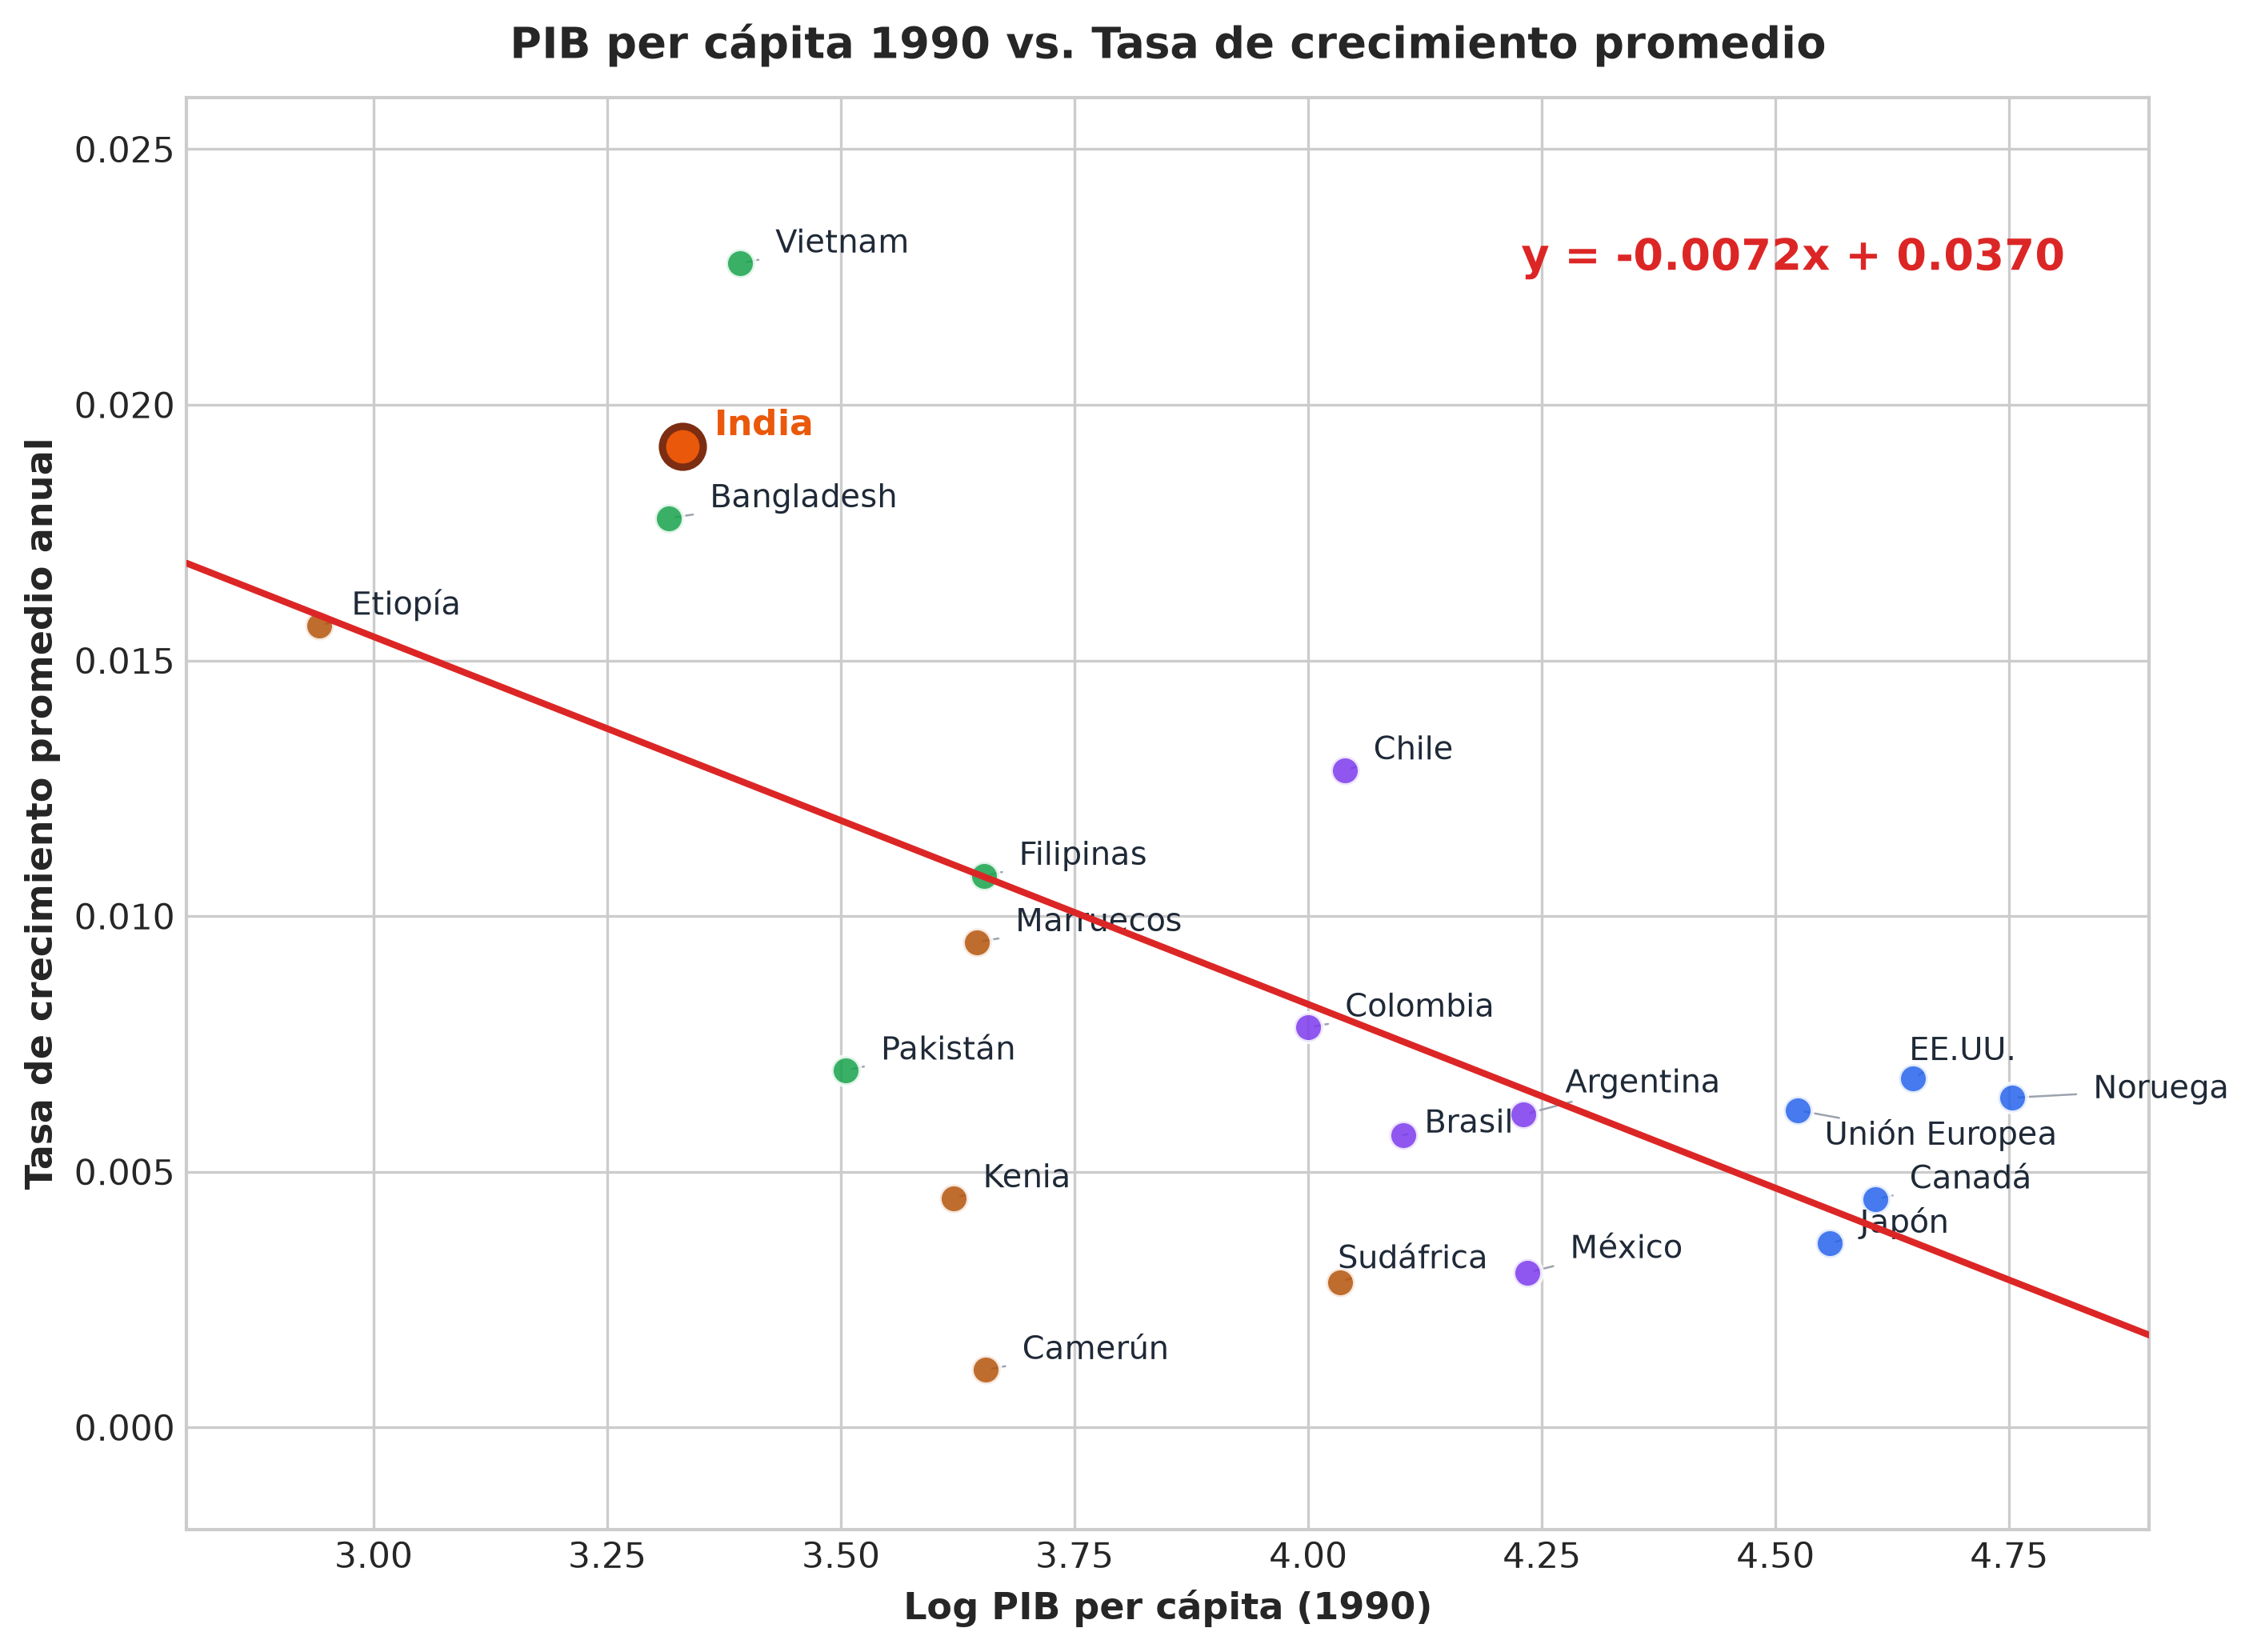
\includegraphics[width=0.88\textwidth]{grafico2_dispersion_logpib90_tasa_promedio.png}
    \caption{Fuente: World Bank (WDI).}
    \label{fig:convergencia_20paises}
\end{figure}

\paragraph{a. ¿La relación estimada es positiva o negativa?}

La relación observada resulta negativa (representada en la recta con pendiente negativa en 0.072, es decir en un 0.72\%, significando que un aumento de un 1\% en el logaritmo del pbi pc deriva en, en promedio, una disminución de 0.72\% en la tasa de crecimiento anual promedio.

\newpage

\paragraph{b. ¿Es compatible con la hipótesis de convergencia absoluta? ¿Qué posición ocupa el país seleccionado respecto de la línea de tendencia? ¿Qué sugiere esto sobre su desempeño relativo al grupo de comparación?}

La información obtenida resulta a favor de la hipótesis de convergencia, debido a que aquellos países con mayor desarrollo en determinado punto de partida (mayor pbi pc en este caso) han sufrido menores tasas de crecimiento anual promedio a lo largo del período mencionado, causando que la ``brecha'' entre países desarrollados y en vías de desarrollo (aquellos con menor pbi pc en el punto de partida y por ende mayores tasas de crecimiento, al menos en promedio) tienda a reducirse.

Respecto a la línea de tendencia, nuestro país (India) observa su situación por encima de ella (AGREGAR DATO DE PUNTO DE PARTIDA EN PBI Y TASA DE CREC PROMEDIO)

Recordando los trabajos prácticos anteriores, podemos mencionar algunas posibles causas de esta mejora india, como por ejemplo el avance de dos sectores claves tales como la industria y los servicios, como también por el desarrollo de factores complementarios, como la generación eléctrica, las redes de comunicación y la conectividad aérea internacional.

\vspace{1em}
\noindent\rule{\textwidth}{0.6pt}
\vspace{0.5em}

\section{Parte 2: Trampas de Pobreza}

\begin{figure}[H]
    \centering
    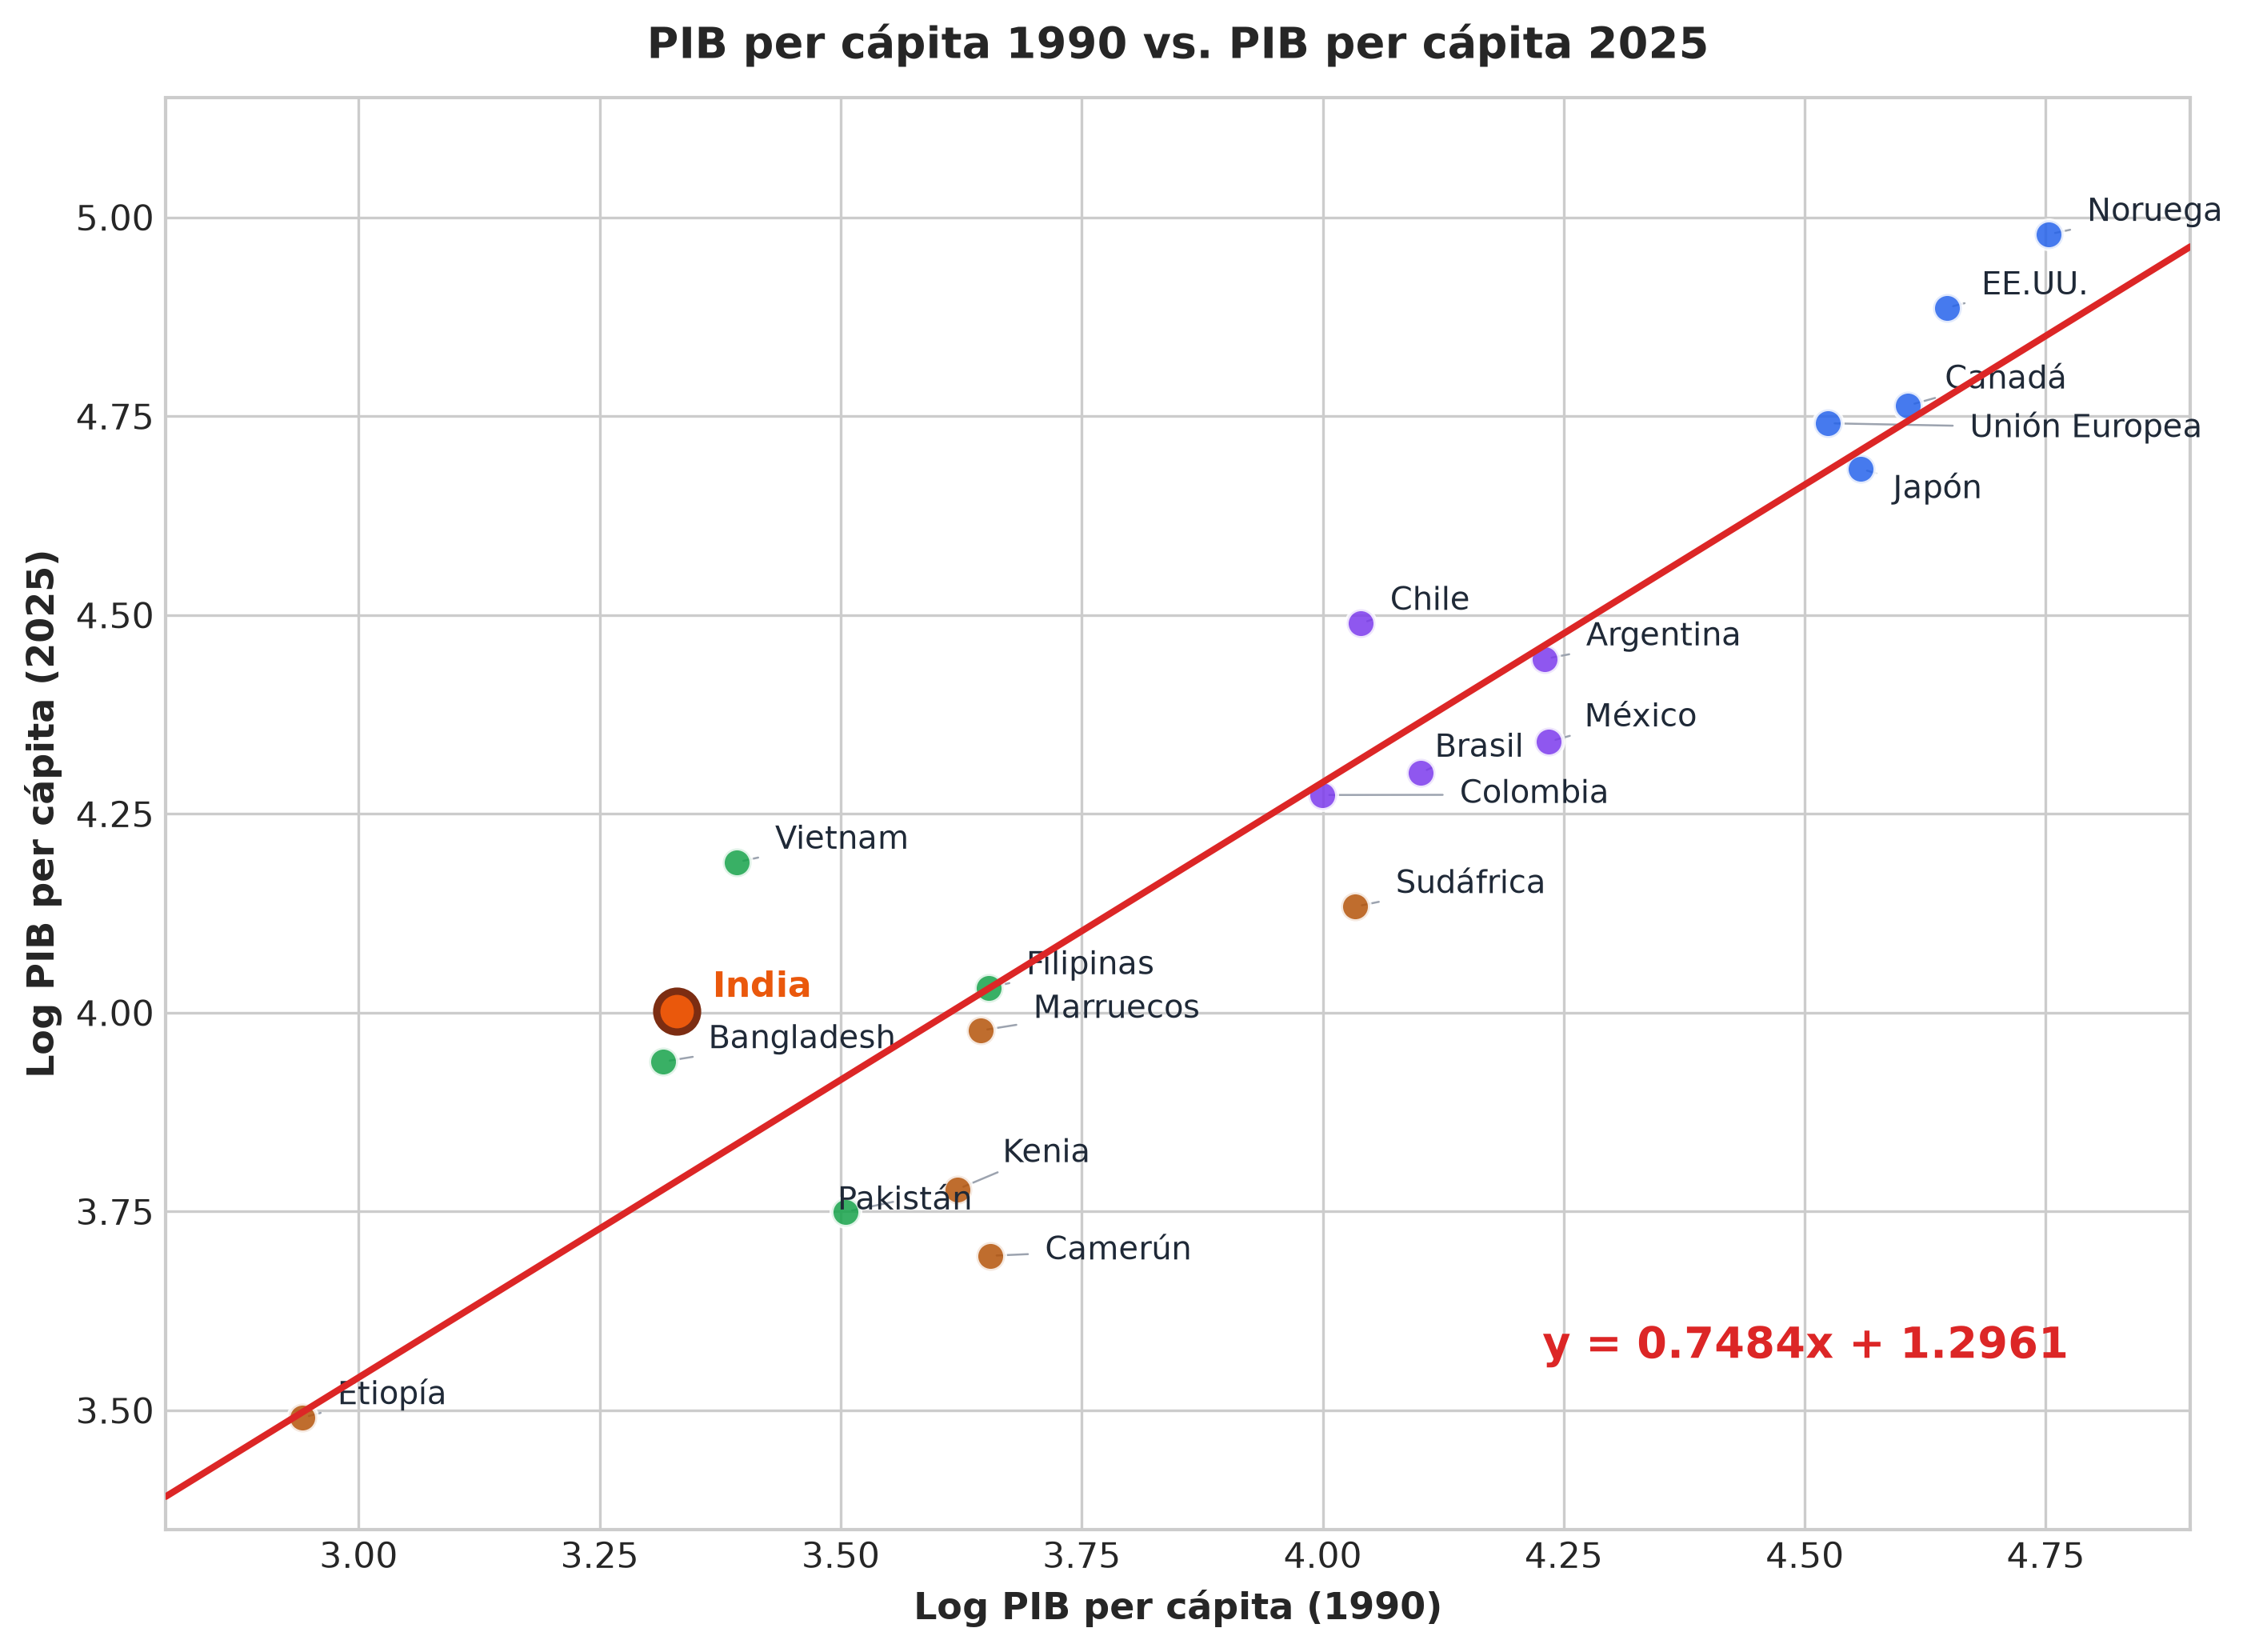
\includegraphics[width=0.88\textwidth]{grafico1_dispersion_logpib90_logpbi25.png}
    \caption{Fuente: World Bank (WDI).}
    \label{fig:pib90_pib25_20paises}
\end{figure}

\paragraph{Comentarios sobre la distribución de los países:}

Todos los países del gráfico están por encima de una recta imaginaria de 45 grados, lo cual demuestra que todas las naciones han mejorado su pbi.

Etiopía se encuentra bastante atrapado en la denominada ``trampa de la pobreza'' aunque de todos modos hemos de mencionar que presenta una cierta mejora. Por otro lado, quien menos creció durante el período fue Camerún con un 0.04

\paragraph{Identificar qué países permanecieron persistentemente en niveles bajos de ingreso. ¿Está tu país en este grupo? ¿Dirías que está en una trampa de pobreza?}

Entre los países que permanecieron en niveles bajos en 1990 están Etiopía, Bangladesh, Pakistán, Camerún, Kenya, y dentro del grupo podemos incluir a India. India se ubica en torno a 3,3 cumpliendo con los términos teóricos de trampa de pobreza, bajo nivel de ahorro y productividad. Hasta esta década India creció un 1\% anual aproximadamente siendo insuficiente para absorber el crecimiento de la población, sin poder reducir la pobreza. A partir de 1991 luego de la crisis de la balanza de pagos, hubo un cambio de rumbo de reformas estructurales.

Analizando los datos para 2025, vemos que India logró aumentar su tas de crecimiento hacia el 4\%, logrando situándose por encima de el promedio de la muestra (la línea celeste), por lo que denota un buen progreso interno, pero que a comparación del resto del gráfico, sigue sin ser una tasa alta,ya que viendo el eje Y, más de la mitad de la muestra de los países se sitúan por encima de India

Cabe destacar que en el gráfico se observa que los países que tienen tasas más altas en 1990, siguen siendo los que tienen tasas más altas en 2025, por lo que la diferencia entre los países de centro y periferia se va agrandando, concordando con la hipótesis de no convergencia

Concluimos que India se encuentra en una trampa de la pobreza, a pesar de su aumento en la tasa de crecimiento respecto a 1990, consideramos que no es suficiente al ver la diferencia en el mismo año con respeto a los demás países.

\newpage
\appendix
\section{Anexo: Evidencia Empírica a Nivel Mundial}

\begin{figure}[H]
    \centering
    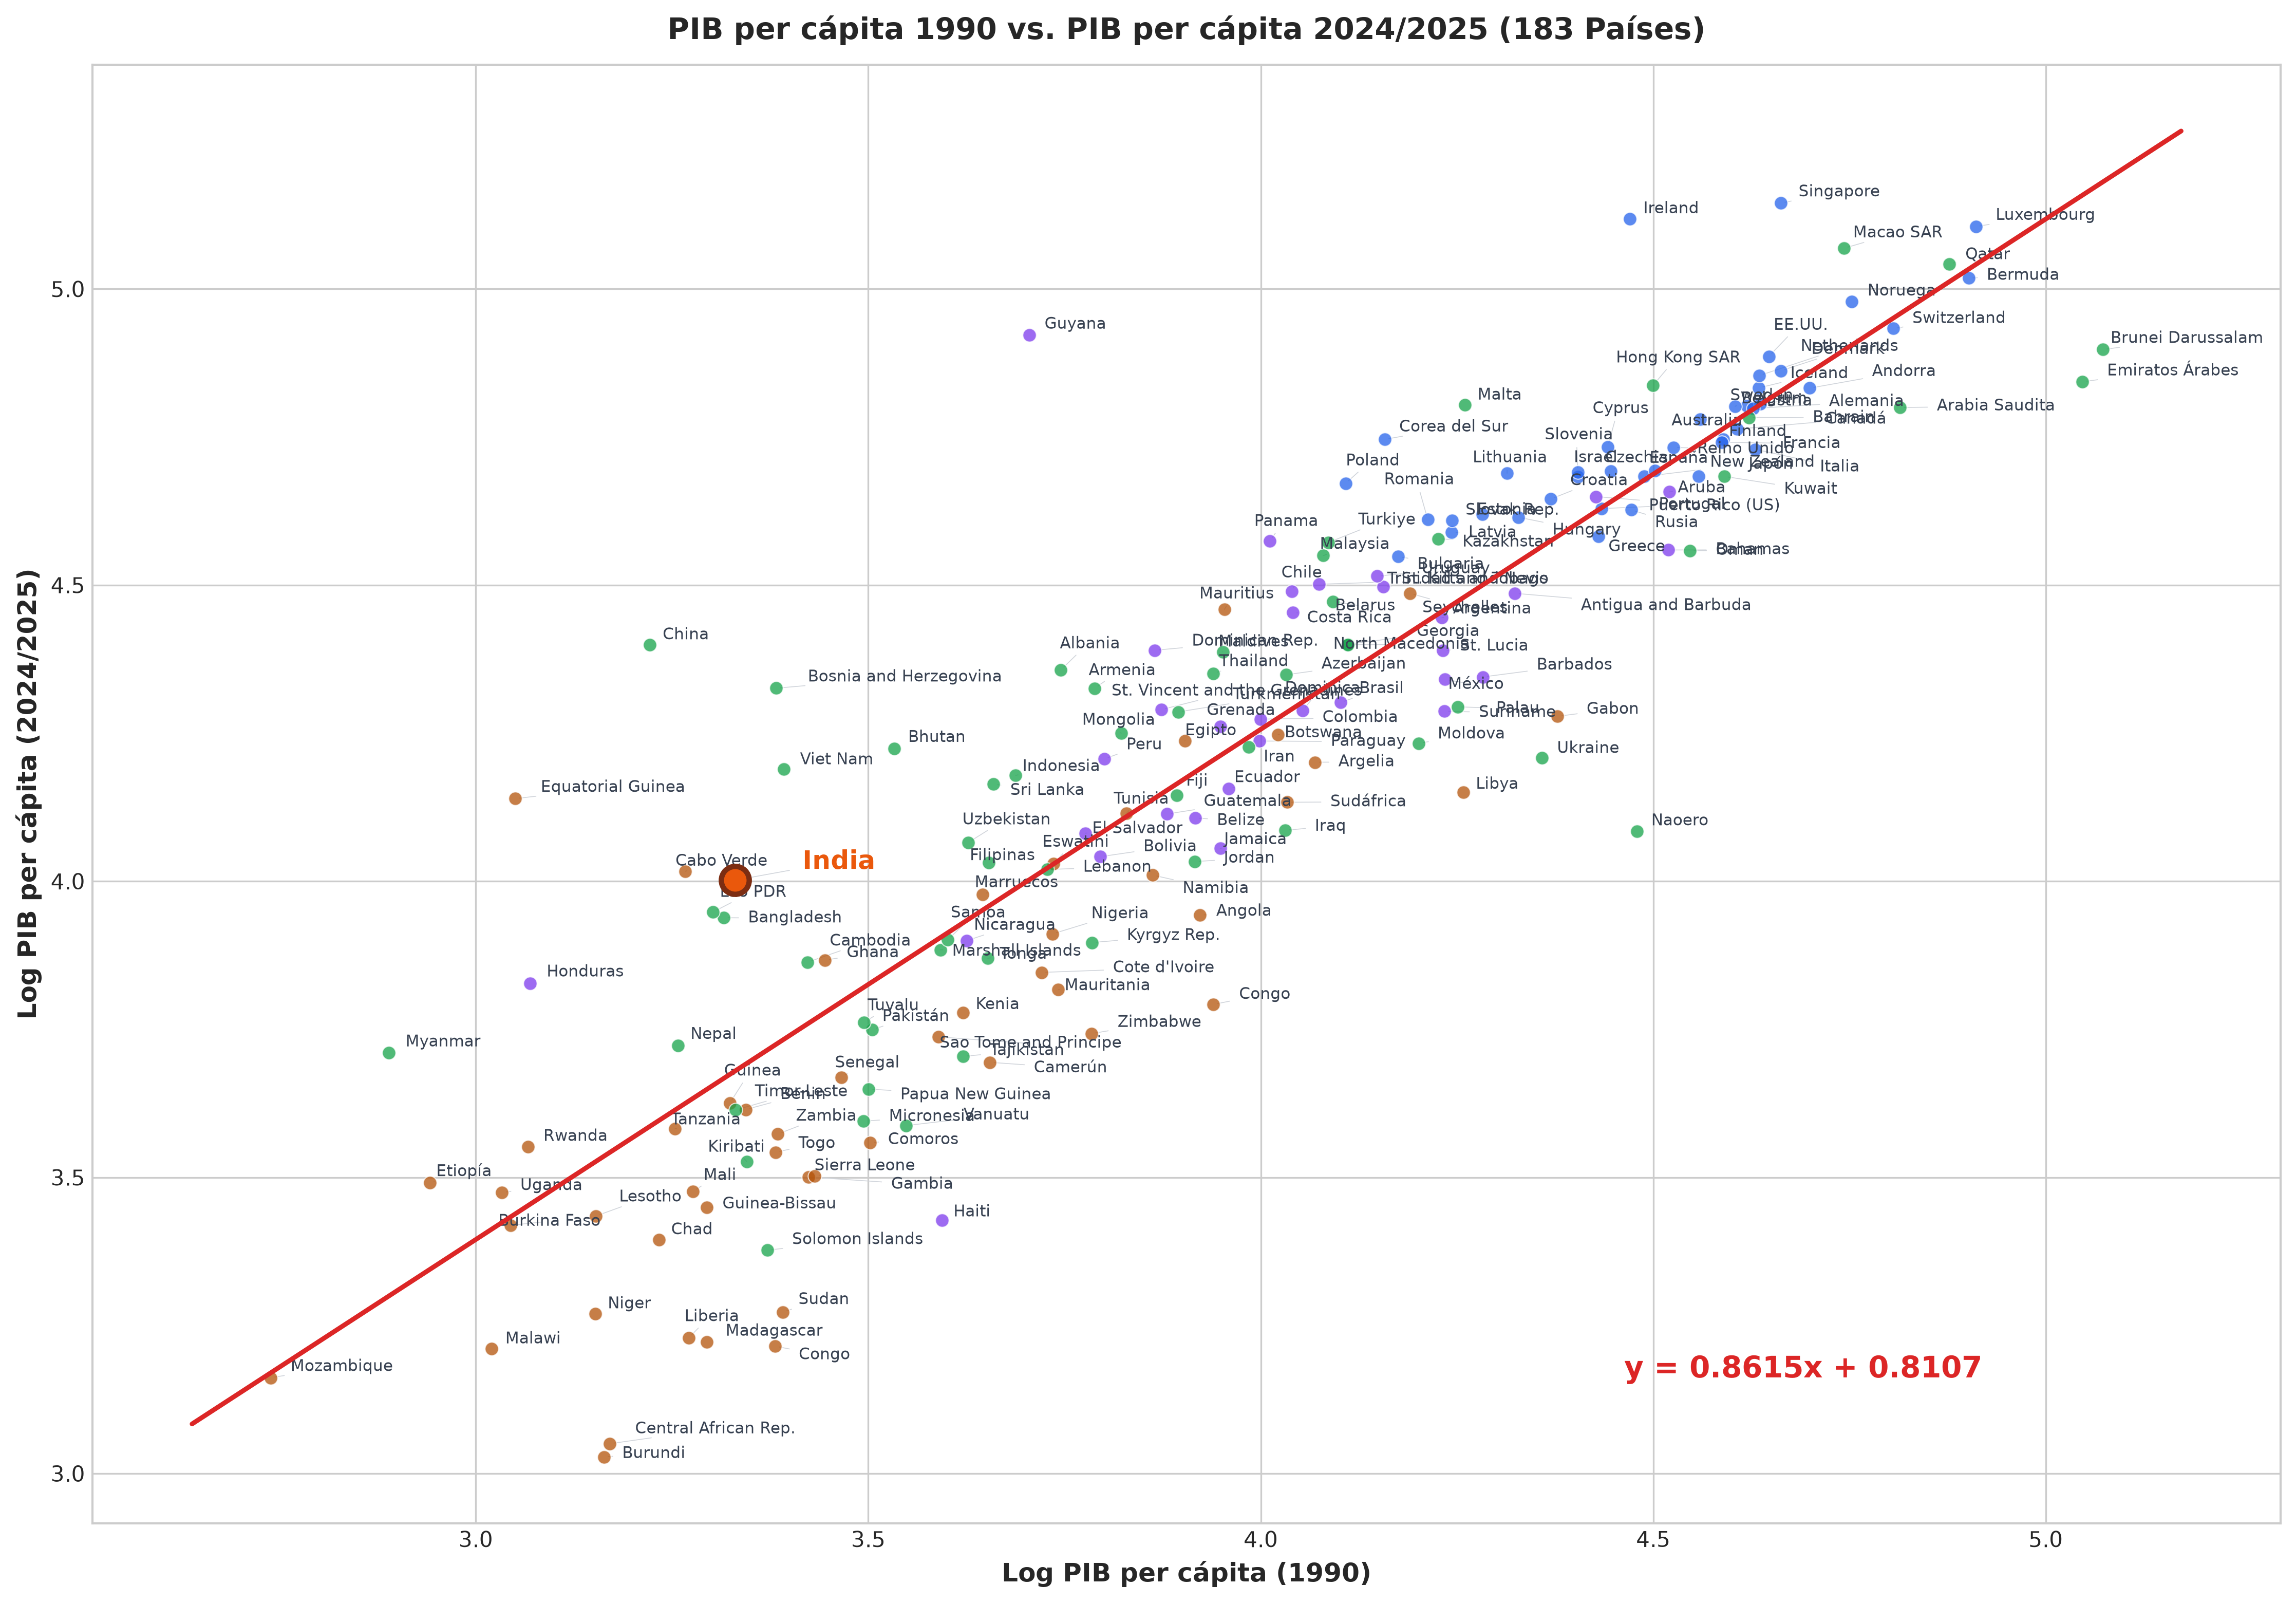
\includegraphics[width=0.88\textwidth]{grafico1_mundial_logpib90_logpbi25.png}
    \caption{Nivel de PIB per cápita inicial (1990) vs. final (2024/2025) para la totalidad de países soberanos con datos disponibles ($N = 183$). Fuente: World Bank (WDI).}
    \label{fig:mundial_niveles}
\end{figure}

\begin{figure}[H]
    \centering
    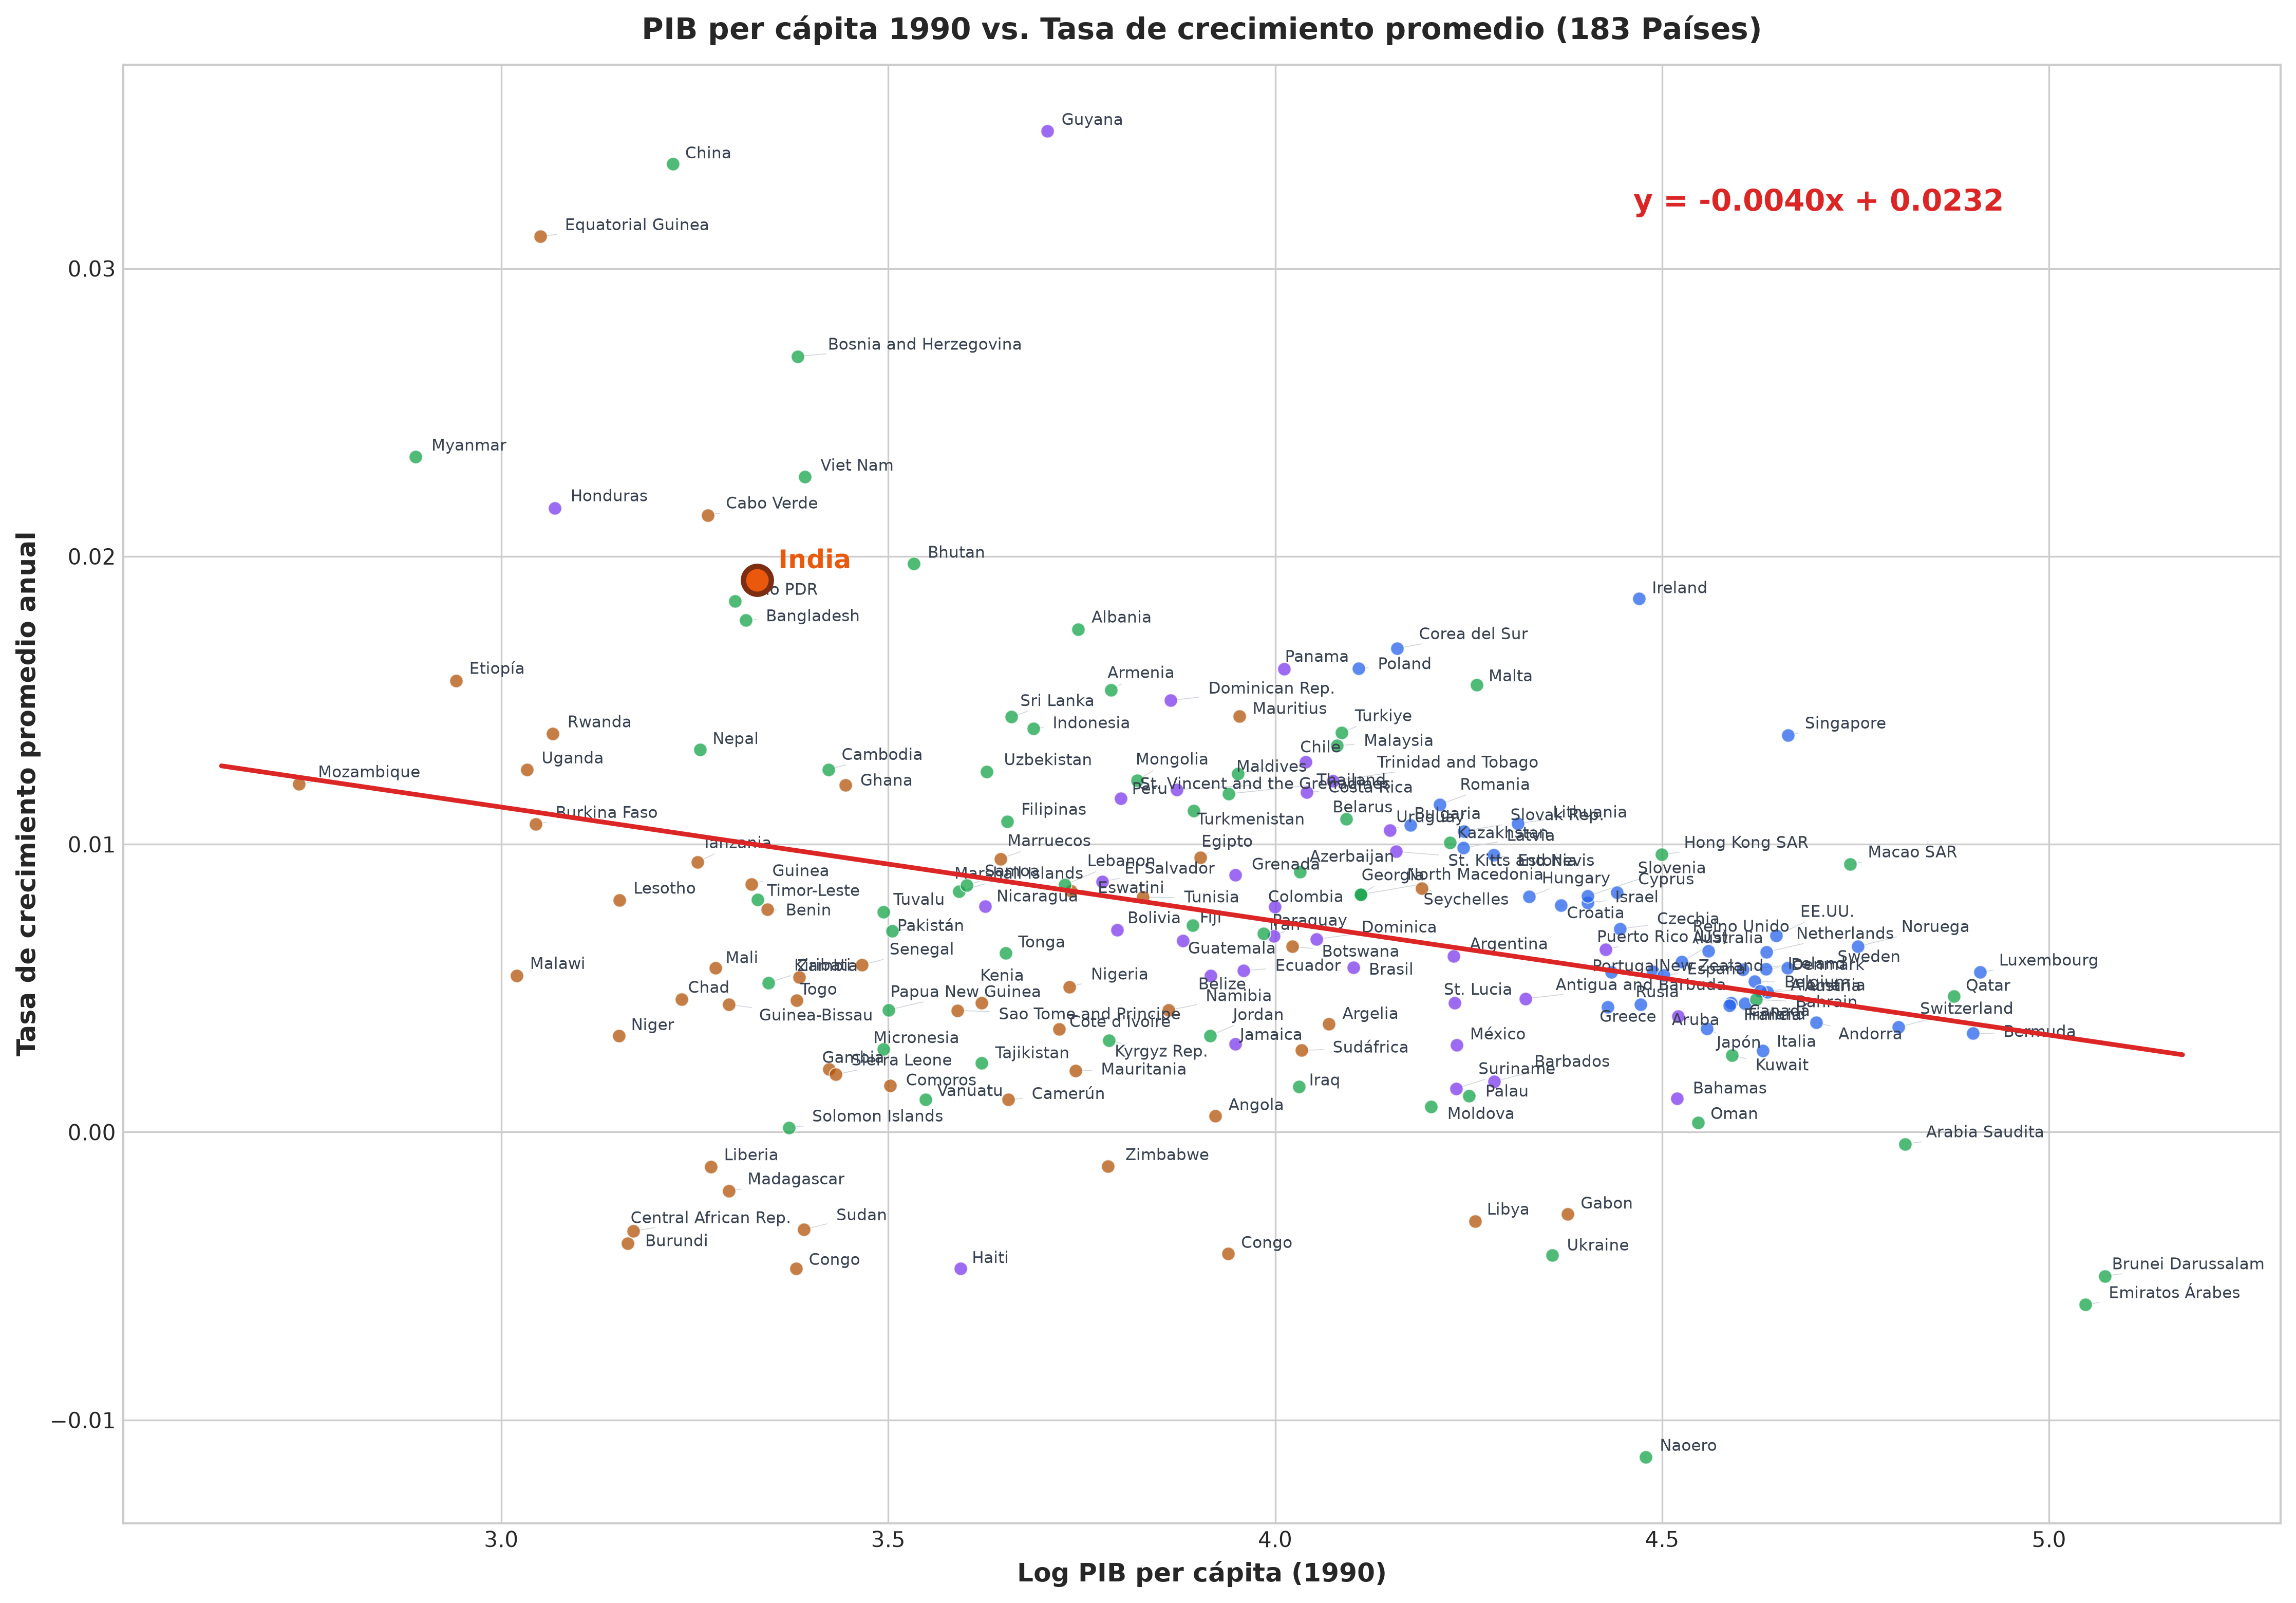
\includegraphics[width=0.88\textwidth]{grafico2_mundial_logpib90_tasa_promedio.png}
    \caption{Convergencia absoluta y tasa de crecimiento anual promedio para la totalidad de países soberanos ($N = 183$). Fuente: World Bank (WDI).}
    \label{fig:mundial_convergencia}
\end{figure}

\end{document}
